\documentclass[12pt]{article}

\usepackage[english]{babel}
% Set page size and margins
% Replace `letterpaper' with`a4paper' for UK/EU standard size
\usepackage[letterpaper,top=2cm,bottom=2cm,left=3cm,right=3cm,marginparwidth=1.75cm]{geometry}
\usepackage{fullpage}
\usepackage{times}
\usepackage{cite}
\usepackage{amsmath}
\usepackage{graphicx}
\usepackage[normalem]{ulem}
\usepackage{fancyhdr,graphicx,amsmath,amssymb, mathtools, scrextend, titlesec, enumitem}
\usepackage[ruled,vlined]{algorithm2e}
\usepackage{romannum}
\usepackage[colorlinks=true, allcolors=blue]{hyperref}
\graphicspath{ {./} }

%

\begin{document}

\begin{titlepage}
\parbox{\linewidth}{
    Names: \underline{Shizhan Liu, Haotian Lu, Ziyi Wang, Haoyuan Zhang}\endgraf\bigskip
    Date: \underline{\today}\endgraf\bigskip
    Course: \underline{ST10701}
}
\parbox{\linewidth}{\centering
    \vspace{5cm}
    \Large \textbf{Secure Automobile Manufacturing and Management}\\
    \vspace{5cm}
}
\parbox{\linewidth}{
    Total in points (100 points total) \underline{\hspace{3cm}}
    \vspace{0.5cm}\par
    Professor's Comments:
}
\end{titlepage}

%

\begin{abstract}
Although the supply chains have been developing at a fast pace recently. 
The United States is still facing some supply chain chaos such as the aspects with product shipment to US, companies
which try to fill orders and consumer demands increase as covid restriction lifts. There are vast areas in which the process can
 be improved. Implementing blockchain related technology with respect to supply chain management allows the product to be tracked, in the order lifecycle, from the beginning to the end, which enable the transparency and efficacy of the management system. The supply chain process includes four different steps: planning and managing the resources needed to meet customer’s demand, choosing supplier to provide goods and services or establishing processes to monitor supplier relationship, organizing activities required to manufacture vehicle, and delivery of orders to customers/car retails. The designed blockchain model includes 2nd tier supplier, 1st tier supplier, warehouses, manufacturer, car maintenance, and car dealership. Using blockchain to manage the supply chain system has several advantages including but not limiting to increase the traceability of the material needed, lower losses from gray market trading and reduce paperwork and administrative cost.
\end{abstract}

%

\section{Introduction}
Automobile manufacturing and management has a gigantic business volume in the US, and it supports numerous employment and GDP in the country.\newline For example, average cars usually have 3000 individual parts. The communication between different parts of the supply chain is important with respect to the production, sells, and customer satisfaction. However, there are several inefficiency and risks with respect to the current supply chain system which includes lack of transparency\cite{choudhurry_2020}, less of 30 percent regard their supply chain as effective, different regulations in different country, and stringent industry standards. This project is looking for a solution for the preceding problems by updating the data on blockchain that is visible among all the parties. By doing so, the barrier between each country has suddenly disappear and the transparency can be largely enhanced. When the goods are transported from one country to another, the data has instantaneously update to the block chain. The blockchain system enhance the product reliability by incorporate an auditor who can audit the information from the blockchain to verify if it is correct. When an certain products shows some faults, the blockchain can locate the position of the problem and fix it in a faster speed.

%

\section{Current Issues} \label{issues}
It is almost impossible for a single industry to fulfill a big order with its own ability. Ever since the first day of the automobile industry, the major industries can't survive without the help of its sub tiers. Once the system grows in such a tremendous trend, the result can be disastrous to the industry.\cite{edi} The major problem of the current automotive industries is the lack of transparency and the track of the order from the main assembly line of the manufacturer, and 30 percent of efficiency is consumed due to over checking the order and painstakingly concern about whether it will be granted on time. Consider the conflict of benefactors between the sub tier manufacturers and the main assembly line. Even after many plants re-opened their doors after shutdowns due to the COVID-19 pandemic, a global shortage of critical vehicle parts like semiconductor chips, tire rubber and foam, forced some automakers to stall vehicle production or have delays in their automobile supply chain. 
\begin{figure}
\centering
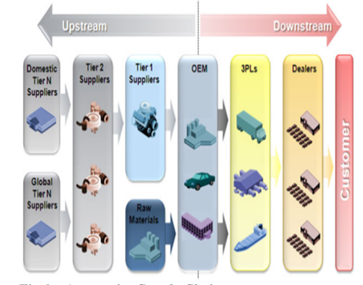
\includegraphics[width=0.8\textwidth]{tiers.png}
\caption{\label{fig:tiers}This Picture of Supply Chain is from Desmond Doran.}
\end{figure}

In such a situation, the meaning of having an efficient cooperation between different parties is extremely crucial. Now solutions about this have already proposed but not satisfied to everyone. IME future introduced a technique to store the data and information about the components in the supply chains stored in form of barcode. However, no matter how to make an agreement, it is difficult to have a common understanding about the current situation.
\begin{figure}
\centering
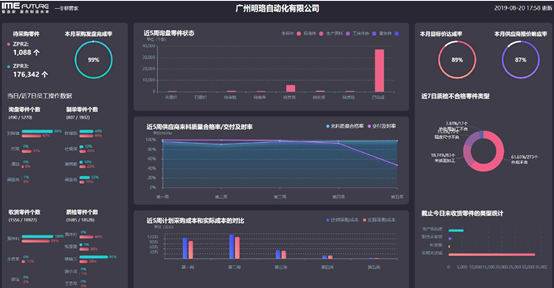
\includegraphics[width=1\textwidth]{efficiency.png}
\caption{\label{fig:efficiency}These data shows the improvement under IME future.}
\end{figure}
As a result of distrust, the companies abroad refuse to use that supply chain system, despite the fact that it improves the on time rate for at least 20 percent. Majorly because its server is located in China. Thus, we believed, in order to keep in pace under such a severe situation, we should do more to secure the basic trust between abroad and domestics enterprise corporators. In such cases, we believe that blockchain\cite{dus} can offer a good solution to balance the relationship between the transparency and efficiency. 


%

\section{Design Solution}
In this section, we introduce the design considerations and outcomes in detail, and present the overall solution to improve the supply chain with blockchain technology.

\subsection{Focal Points}
As mentioned in the section \ref{issues}, we focus on the sourcing and delivering process of the supply chain, and try to present a solution that can reduce the number of unqualified products and reduce the effort to maintain a timely product delivery. First of all, unqualified products has been a lasting issue for the automobile supply chain industry according to the Blume report \cite{blume}, and has negative effect on both the credibility and profit of the companies involved. Sometimes, a concealed unqualified product will eventually make its way to the final production car, and even threaten the safety of the passengers. Second, on-time delivery of products is also crucial since the chain of production will halt if certain tier of car parts fails to be delivered on time for assembly. For example, there is a global shortage of smart chips on cars, and delayed delivery is severely affecting the profits of many car manufacturing companies \cite{shortage}.

\subsection{Blockchain Technology}
In order to deal with the problems, we propose to use blockchain technology considering the following aspects.
\begin{itemize}
    \item Multiple parties are involved in the supply chain, namely customers, dealership, distributors, investors, manufacturers, car service, supervisors and suppliers. They are individual parties that act on behalf of their profits, so trusting and cooperation is usually done using contracts that process legal forces.
    \item Supply chain products rely heavily on contractual relationships and value exchange, and contracts with predefined logic can be managed digitally and executed automatically, as long as the conditions are met. This is exact use case for smart contracts.
    \item Assets like credit and due payments and can be transferred and managed digitally.
    \item Function of individual parties has to be controlled so that the risk of disallowed access can be reduced,
    \item This is a need for shared write access to an order during its lifecycle, specifically dealing with the creation, progression, finalization and clearance.
\end{itemize}
Considering the requirements above, blockchain technology evaluated to be effective in the supply chain system.


%

\section{Implementation}
In this part, we elaborate on the process of implementation and the contract code. We first introduce the entity modeling which represents the actual parties and their roles in the supply chain, and briefly include their abilities. Then, we introduce the order system on the platform in detail, which represents the exchange place for value and products. Lastly, we introduce the token system that adheres to ERC721 with modifications and upgrades for advanced properties.

\subsection{Entity}
There are 8 entity roles in the system, namely
\begin{enumerate}[label=\alph*.]
    \item Customer
    \item Dealership
    \item Distributor
    \item Investor
    \item Manufacture
    \item Service
    \item Supervisor
    \item Supplier
\end{enumerate}
\begin{figure}[h]
    \centering
    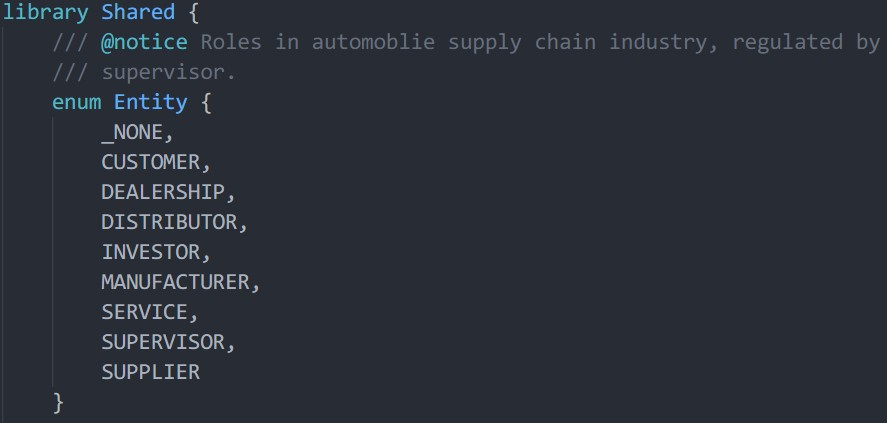
\includegraphics[width=0.75\textwidth]{entities.jpg}
    \caption{Entity roles}
    \label{fig:entity}
\end{figure}
They make up the supply chain ecosystem and have their controlled access to the system respectively. For instance, the dealership takes authorized sales privilege from manufacturers and then sell the cars to customers. More, the customers can take the car to service for maintenance, where the service will verify the validity of car parts. Besides, the suppliers and manufacturers can create and take orders from the system as long as they have enough margins put forward for the specified order. In addition, investor may come in for car parts that highly valuable in the later sales, or sell parts for a profit.

\subsection{Order}
The order system is applied for registered parties in the system, and require a ratio to the price of the final payment put forward, also known as margins. The detailed procedure of the order system is illustrated as follows. First, an entity makes an order for a specific product by calling the function createOrder and put forward a margin for the order. The order also comes with a due. Before anyone takes the order, the entity is allowed to cancel the order. Then, a supplier takes the order and tries to fill it within the due specified. Once filled, the filler can mark the order as filled and send it to the distributor/warehouse for product pickup. Once the order creator confirms the product received, the order creator sends the final payment and the platform clears the deal.

\subsection{Token}
The product or car parts can be minted to a digital token and transferred between entities, because it strictly follows the ERC721 token standards. The token also comes with source tracing by implementing a mapping to a dynamic array of its parent car parts.

%

\section{Conclusion}
During this trying time, COVID had significantly disrupted the supply chain of different automotive manufacturing companies. There is a dire need of solutions for the long-existing problem in the automotive supply chain industry. The main issues the Secure Automobile manufacturing and management blockchain addresses are the lack of transparency and faulty parts. As we upload the production and movement of parts onto the blockchain. We are able to trace parts and vehicles manufactured all the way from 2nd tier supplier to car dealership. This information can be made available to independent auditors, who are also participants on the blockchain, for auditing purposes; as well as the public such that public trust can be built into this company. With the involvement of auditors, faulty parts are less likely going to make it into the production line and create hazards further down the line. Furthermore, this system can be integrated with IoT sensors such that information can be uploaded onto the blockchain automatically without human involvement, which drastically increases efficiency. However, due to the limited functionality of this blockchain, we are unable to help resolve other issues in the automotive supply chain industry, including forecasting demands, inventory mismanagement, and others. Nonetheless, the involvement of other technologies such as A.I. can be part of the solution to these problems.

\pagebreak

\bibliographystyle{IEEEtran}
\bibliography{cite.bib}


\end{document}


% \begin{enumerate}
% \item Like this,
% \item and like this.
% \end{enumerate}
% \dots or bullet points \dots
% \begin{itemize}
% \item Like this,
% \item and like this.
% \end{itemize}

% \begin{figure}
% \centering
% \includegraphics[width=0.3\textwidth]{frog.jpg}
% \caption{\label{fig:frog}This frog was uploaded via the file-tree menu.}
% \end{figure}

% \begin{table}
% \centering
% \begin{tabular}{l|r}
% Item & Quantity \\\hline
% Widgets & 42 \\
% Gadgets & 13
% \end{tabular}
% \caption{\label{tab:widgets}An example table.}
% \end{table}

% \LaTeX{} is great at typesetting mathematics. Let $X_1, X_2, \ldots, X_n$ be a sequence of independent and identically distributed random variables with $\text{E}[X_i] = \mu$ and $\text{Var}[X_i] = \sigma^2 < \infty$, and let
% \[S_n = \frac{X_1 + X_2 + \cdots + X_n}{n}
%       = \frac{1}{n}\sum_{i}^{n} X_i\]
% denote their mean. Then as $n$ approaches infinity, the random variables $\sqrt{n}(S_n - \mu)$ converge in distribution to a normal $\mathcal{N}(0, \sigma^2)$.